\section{John Joseph O'Brien}

\MainPerson{John Joseph\textsuperscript{3} O'Brien} (\Lineage{2}{John}, \Lineage{1}{William}) was born in Boston, Suffolk County, Massachusetts, on 29 January 1861.\cite{John3OBrienBirth} He was baptized at St. John the Baptist Church in Boston on 1 February 1861.\cite{John3OBrienBaptism} He died in Brookline, Norfolk County, Massachusetts, on 15 May 1938.\cite{John3OBrienDeath} He is buried at Mt.\ Calvary Cemetery, Boston.\cite{John3OBrienBurial} He married, at St. Augustine Church in Boston on 6 February 1890, \MainPerson{Emma A.\ Mahony}.\cite{John3OBrienMarriage,John3OBrienMarriage2} Emma was born in Boston on 27 September 1862 to Edward Mahony and Catherine Josephine Kenney.\cite{EmmaMahonyBaptism} She died in Brookline on 11 July 1950.\cite{EmmaMahonyDeath}

John's father died in 1863\cite{John2OBrienDeath} and his mother married Thomas Bowser in 1867.\cite{MaryMahoneyBowserMarriage} Sometime between 1870 and 1876, the family moved from Hanover St.\ in the North End to Hudson St.\ in Boston's South Cove neighborhood.\cite{ThomasBowser1870,ThomasBowser1876} The family later relocated to 45 Court St.\ in Medford, Middlesex County, Massachusetts, and remained there for many years.\cite{Census1910John3OBrien,Census1930John3OBrien}

John worked as a picture frame manufacturer.  He took over the business from the previous owner, B.\ Ferdinand Sargent, when Sargent relocated to Minnesota in 1881 or 1882.\cite{PictureFrameLabel, Sargent} John continued running the business until about 1917.\cite{John3OBrien1916} The frame shop occupied the second floor of the building at 69 Cornhill in Boston.\cite{John3OBrien1916,FrameShopFire} 

\begin{figure}
\centering
\includegraphics[width=\textwidth]{picture_frames_label}
\caption{Label for John J.\ O'Brien, picture frames, 69 Cornhill, Boston, Mass., undated. Historic New England, Ephemera Collection, GUSN-265637 (\url{http://gusn.us/265637}).}
\end{figure}

\begin{figure}
	\centering
	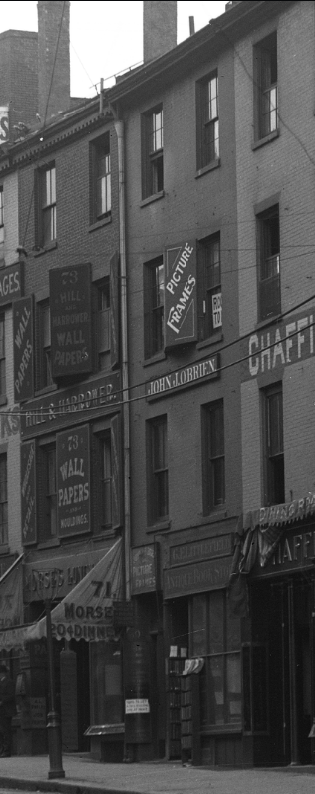
\includegraphics[height=0.8\textheight]{picture_frame_shop}
	\caption{John J.\ O'Brien's frame shop at 69 Cornhill, Boston. Detail from ``Crosswalk on Corn Hill opposite Franklin Avenue, looking west, sect. 8 1/2, Boston, Mass.,'' photograph, Boston Transit Commission, 14 Apr 1897, John Booras collection of plate glass negatives, Historic New England, GUSN-318238 (\url{http://gusn.us/318238}) }
\end{figure}

Cornhill was a street located at what is now the Government Center complex. At its heyday, many booksellers and publishers located themselves on Cornhill and it became known as one of Boston's intellectual centers.\cite{Cornhill} The street was mostly destroyed during the city's urban renewal phase in the 1960s. The only remnants of the original Cornhill are the Sears Block and Sears Crescent (location of the famous ``steaming teakettle'').\cite{Cornhill} 

A fire in 1904 caused major damage to John's frame shop, mostly from the water used to put out the fire. Efforts to fight the fire were complicated by an avalanche of snow falling off the roof and nearly burying the firefighters, and an intoxicated man trying to help by climbing the stairs of the building and hanging onto the firehose.\cite{FrameShopFire} John was able to recover the business and continued operating out of this location until at least 1916.\cite{John3OBrien1916}

John, his wife Emma, and several of their children are buried in the Mahony/Mahoney plot owned by Emma's father Edward at Mt.\ Calvary Cemetery in Boston's Roslindale neighborhood.\cite{John3OBrienBurial}

\begin{KidsIntro}
	Children of John Joseph\textsuperscript{3} O'Brien and Emma A.\ (Mahony) O'Brien:
\end{KidsIntro}

\begin{Kids}
	\KidNum{}{i.}\KidName{Mildred Loretta\textsuperscript{4} O'Brien}, b.\ 14 Nov.\ 1890;\cite{Mildred4OBrienBirth} d.\ 26 May 1891.\cite{Mildred4OBrienDeath}
	
	\KidNum{\ref{per:Francis4OBrien}}{ii.}\KidName{Francis Joseph O'Brien}, b.\ 2 April 1892; m. Malden, Middlesex C., Mass., 12 Sept.\ 1921, \KidName{Mary Helena Flynn}.
	
	\KidNum{\ref{per:Pauline4OBrien}}{iii.}\KidName{Pauline M.\ O'Brien}, b.\ 9 June 1894; m.\ 9 June 1930, \KidName{Charles Lucius Baine}.
		
	\KidNum{\ref{per:Mildred4OBrien}}{iv.}\KidName{Mildred Louise O'Brien}, b.\ 29 Sept.\ 1896; m.\ Medford, Middlesex Co., Mass., Feb.\ 1925, \KidName{Albert Joseph French}.
	
	\KidNum{}{v.}\KidName{Edward O'Brien}, b.\ Medford, 5 July 1898;\cite{Edward4OBrienBirth} d.\ Medford, 24 Dec.\ 1898.\cite{Edward4OBrienDeath}
	
	\KidNum{}{vi.}\KidName{Almyra Louise O'Brien}, b.\ Medford, 27 June 1901;\cite{Almyra4OBrienBirth} d.\ Medford, 13 July 1902.\cite{Almyra4OBrienDeath}
\end{Kids}
